% !TeX root = Report.tex
\documentclass[12pt]{article}

% Package imports (organized and deduplicated)
\usepackage{biblatex}
\usepackage{changepage}
\usepackage{color}
\usepackage{enumitem}
\usepackage{float}
\usepackage{graphicx}
\usepackage{listings}
\usepackage{sectsty}
\usepackage{xcolor}
\usepackage[breaklinks=true]{hyperref}
\usepackage{xurl}
\usepackage{tikz}
\usepackage{lipsum}
\usepackage[format=plain,
            labelfont=it,
            textfont=]{caption}
\usetikzlibrary{shapes.geometric, arrows, positioning, calc}
\usepackage{./timing-diagrams}
\usetikzlibrary{calc}
\setcounter{biburlnumpenalty}{100}
\setcounter{biburlucpenalty}{100}
\setcounter{biburllcpenalty}{100}

\newcommand{\subsubsubsection}[1]{\paragraph{#1}\mbox{}\\}
\setcounter{secnumdepth}{4}
\setcounter{tocdepth}{4}

\newcommand{\writersnote}[1]{\marginpar{\small{\textcolor{blue}{Writer's note:}} \scriptsize\textit{#1}}}

% \usepackage{background}
% \backgroundsetup{
%   position=current page.north west,
%   angle=0,
%   nodeanchor=north west,
%   vshift=-1cm,
%   hshift=1cm,
%   color=red,
%   opacity=1,
%   scale=1,
%   contents={Preprint}
% }

\definecolor{darkblue}{RGB}{0, 0, 102} 
\hypersetup{
    colorlinks=true,
    pdfborder={0 0 0},
    linkbordercolor=white,
    urlcolor=darkblue,
    linkcolor=darkblue,
    citecolor=darkblue,
    filecolor=darkblue
}

% Make bibliography ragged right instead of justified
\AtBeginDocument{
  \renewcommand{\bibsetup}{\raggedright}
}
% Document configuration
\restylefloat{table}
\graphicspath{{./images/}}
\addbibresource{Library.bib}
\subsectionfont{\fontsize{12}{14}\selectfont}

% Author information
\author{
    Group Number: 107\\
    Joar Heimonen, Christian Vu, Naly Keli \\
    \texttt{contact@joar.me}\\ 
    \texttt{chvu002@student.kristiania.no}\\
    \texttt{nake002@student.kristiania.no}
}

% Title configuration
\title{
  \textbf{Preliminary Title}\\
  \large{Preliminary Description}
}
\date{\today}

\newcommand{\license}{
    \vspace{1em}
    \noindent\small{© 2025 Joar Heimonen,  Christian Vu, Naly Keli\\
    This work is licensed under a \href{https://creativecommons.org/licenses/by-sa/4.0/}{Creative Commons Attribution-Sharealike 4.0 International License}.}
}
\begin{document}
\maketitle

\begin{abstract}
  Preliminary Abstract
\end{abstract}

\pagebreak

\tableofcontents

\pagebreak


\section{Introduction}
There are many paradigms of commercial sensor management and monitoring. Organizations can use anything from 
PLC (programmable Logic Controllers) to IoT devices to manage and monitor their sensors. For commercial use 
some of these alternatives are more popular than others. There are also a large amount of different higher level protocols
like MQTT, HTTP and SNMP that can be used to manage and monitor sensors. We propose using the NETCONF protocol 
with YANG sensor models for management. This work will be done in collaboration with Lightside Instruments AS.

\writersnote{
  unprecise, replace: "can use anything from..." and all other vague statements.
}

This document will cover the following three topics:
\begin{itemize}
  \item \textbf{Work Methodology:} An indept analysis of the knowledge base around work methods like Scrum, Kanban, and Waterfall. 
  With a focus on how our work methodology differs from these.
  \item \textbf{NETCONF and YANG sensor management}: A qualitative analysis of the NETCONF and YANG protocols and how they can be used to manage sensors.
  \item \textbf{NETCONF Security}: A qualitative analysis of the security aspects of the NETCONF protocol.
\end{itemize}

\section{Lightside Instruments AS}
Lightside Instruments is a company specializing in developing instruments with model based network management 
for use in networking, network interconnect testing and telemetry. 
They design their instruments with YANG (RFC7950) \cite{bjorklundYANG11Data2016} models and NETCONF (RFC6241) \cite{ennsNetworkConfigurationProtocol2011} protocol. 
The instruments are based on IETF standards and drafts, 
and are implemented with software tools available in Debian, programmable 
logic and open hardware \cite{LightsideInstrumentsYANG}.

\section{Technical background}

\subsection{NETCONF and YANG}
NETCONF \cite{ennsNetworkConfigurationProtocol2011} is a model based Network Configuration Protocol.
Each NETCONF device presents the aquiring device with a YANG \cite{bjorklundYANG11Data2016} data model
consisting of the device state and parameters. 
Each data model has a set of constraints making them error correcting.

\subsection{Node-RED}
Node-RED \cite{LowcodeProgrammingEventdriven} is an open source low code programming tool for event driven applications.
It is developed by IBM and is based on Node.js \cite{NodejsRunJavaScript}.
Node-RED is used to connect hardware devices and APIs through a visual programming interface.

\subsection{Grafana}
Grafana \cite{GrafanaOpenComposable} is an open source data visualization tool.
It is used to visualize arbitrary data from different data sources.

\subsection{Scrum}
Scrum \cite{HomeScrumorg} is a framework for agile \cite{AgileSoftwareDevelopment2025} software development.

\subsection{Kanban}
Kanban \cite{Kanban2025} is a framework for agile software development.

\subsection{Waterfall}
Waterfall \cite{WaterfallModel2025} is a framework for software development.

\subsection{Extreme Programming}
Extreme Programming \cite{ExtremeProgramming2025} is a framework for agile software development.

\section{Work Methodology}

\subsection{Research Question}
This review examines the claims that Scrum, Kanban, Waterfall, Extreme Programming and DevOps 
increases worker productivity substantiated by empirical evidence.

\subsection{Scoping Review}

\subsubsection{Search strategy}
The following is our search strategy for the scoping review.
We will be searching for quantitative studies on the efficiency of the following work methodologies:
\begin{itemize}
  \item Scrum
  \item Kanban
  \item Waterfall
  \item Extreme Programming
  \item DevOps
\end{itemize}
We will be searching the following databases:
\begin{itemize}
  \item IEEE Xplore \cite{IEEEXplore}
  \item ACM Digital Library \cite{ACMDigitalLibrary}
  \item Google Scholar \cite{GoogleScholar} (Meta database)
\end{itemize}
We will also be searching the following industry websites:
\begin{itemize}
  \item Agile Alliance \cite{AgileAlliance2015}
  \item Scrum.org \cite{HomeScrumorg}
  \item DevOps Institute \cite{Organisations}
  \item Scrum Alliance \cite{ScrumAllianceFind}
\end{itemize}
\writersnote{
  This section becomes a bit monotone, consider fewer lists.
}
Our search will consists of a set of primary and secondary keywords.
The primary keywords are:
\begin{itemize}
  \item Scrum
  \item Kanban
  \item Waterfall
  \item Extreme Programming
  \item DevOps
\end{itemize}
The secondary keywords are:
\begin{itemize}
  \item Effectiveness
  \item Efficiency
  \item Productivity
  \item Performance
  \item Success
  \item Failure
\end{itemize}
The search will be done using the following search string:

\begin{adjustwidth}{-4em}{0pt}
\begin{verbatim}
       (Scrum OR Kanban OR Waterfall OR "Extreme Programming" OR DevOps) 
                                      AND
(Effectiveness OR Efficiency OR Productivity OR Performance OR Success OR Failure)
\end{verbatim}
\end{adjustwidth}

\subsubsection{Exclusion Criteria}
The systematic review will include articles meeting the following criteria:
\begin{itemize}
  \item Published after January 1, 2020
  \item Published in English
  \item Relevant to the research question
  \item Empirical evidence
  \item Quantitative studies
  \item One of the 20 first results from each database
  \item Evaluating the effectiveness of the following methodologies:
  \begin{itemize}
    \item Scrum
    \item Kanban
    \item Waterfall
    \item Extreme Programming
    \item DevOps
  \end{itemize}
\end{itemize}

\subsubsection{Result}
After applying the exclusion criteria to a set of 60 articles, we discovered that 4 of them were duplicates.
The 56 remaining articles were screened by title and abstract, resulting in 12 articles being excluded.
The 44 remaining articles were assessed for eligibility, resulting in 33 articles being excluded.
The 11 remaining articles were included in the review.

\subsubsubsection{PRISMA flow diagram}
\textit{Figure \ref{fig:prisma}} shows the PRISMA \cite{PRISMAStatement} flow diagram for the scoping review.
The PRISMA flow diagram is a standardized way of reporting the results of a scoping review.

\begin{figure}
  \centering
  \begin{adjustwidth}{-4em}{0pt}
  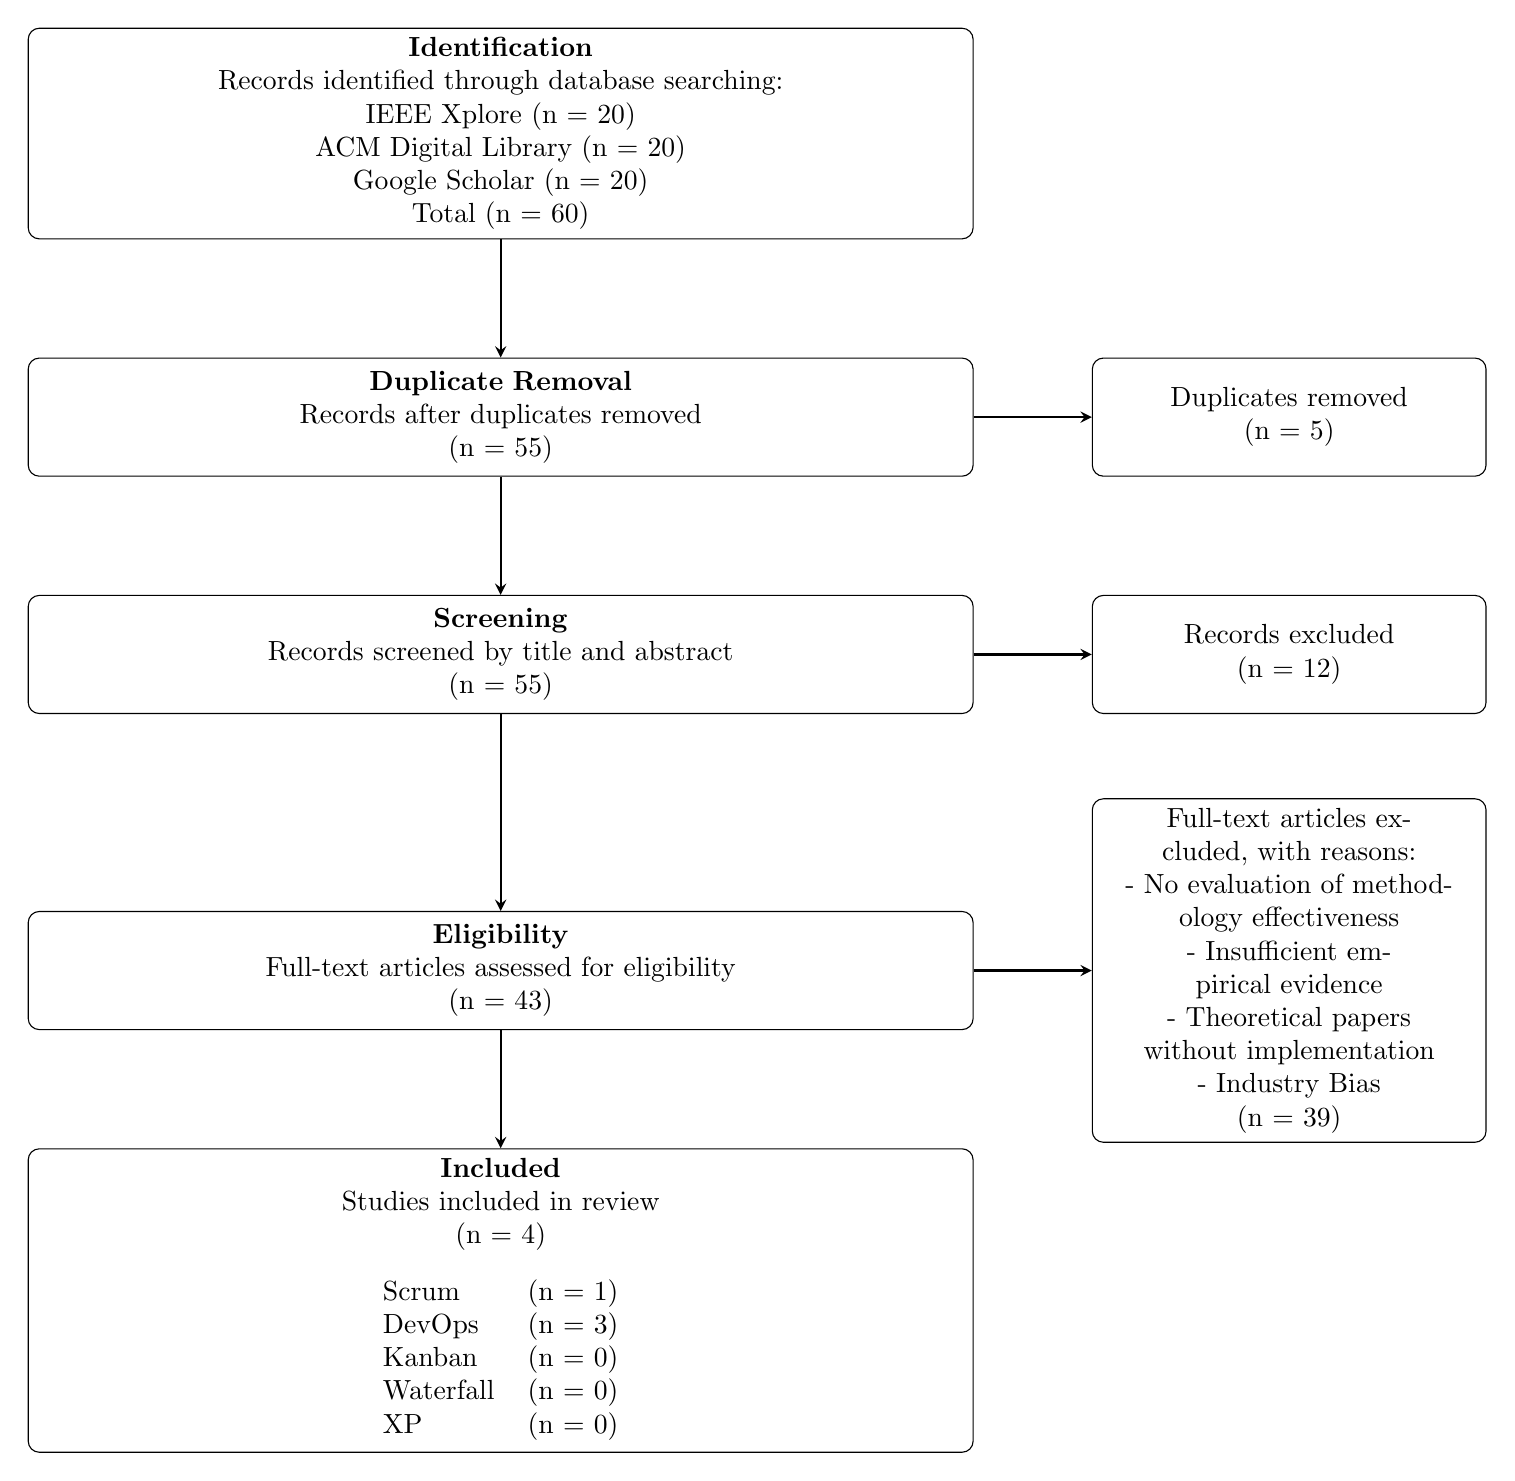
\begin{tikzpicture}[
   node distance = 1.5cm,
   box/.style = {draw, rectangle, rounded corners, minimum width=12cm, minimum height=1.5cm, text width=11.5cm, align=center},
   sidebox/.style = {draw, rectangle, rounded corners, minimum width=5cm, minimum height=1.5cm, text width=4.5cm, align=center},
   line/.style = {draw, -stealth, thick}
   ]
  % Identification box
  \node[box] (identification)
   {\textbf{Identification} \\
   Records identified through database searching:\\
   IEEE Xplore (n = 20)\\
   ACM Digital Library (n = 20)\\
   Google Scholar (n = 20)\\
   Total (n = 60)};
  
  % Duplicates removal box
  \node[box, below=of identification] (duplicates)
   {\textbf{Duplicate Removal} \\
   Records after duplicates removed\\
   (n = 55)};
  \node[sidebox, right=1.5cm of duplicates] (excluded0)
   {Duplicates removed\\
   (n = 5)};
  
  % Screening boxes
  \node[box, below=of duplicates] (screening)
   {\textbf{Screening} \\
   Records screened by title and abstract\\
   (n = 55)};
  \node[sidebox, right=1.5cm of screening] (excluded1)
   {Records excluded\\
   (n = 12)};
  
  % Eligibility boxes
  \node[box, below=2.5cm of screening] (eligibility)
   {\textbf{Eligibility} \\
   Full-text articles assessed for eligibility\\
   (n = 43)};
  \node[sidebox, right=1.5cm of eligibility] (excluded2)
   {Full-text articles excluded, with reasons:\\
   - No evaluation of methodology effectiveness\\
   - Insufficient empirical evidence\\
   - Theoretical papers without implementation\\
   - Industry Bias\\
   (n = 39)};
  
  % Included box
  \node[box, below=of eligibility] (included)
   {\textbf{Included} \\
   Studies included in review\\
   (n = 4)\\[0.3cm]
  \begin{tabular}{ll}
   Scrum & (n = 1)\\
   DevOps & (n = 3)\\
   Kanban & (n = 0)\\
   Waterfall & (n = 0)\\
   XP & (n = 0)
  \end{tabular}};
  
  % Arrows
  \draw[line] (identification) -- (duplicates);
  \draw[line] (duplicates) -- (screening);
  \draw[line] (screening) -- (eligibility);
  \draw[line] (eligibility) -- (included);
  \draw[line] (duplicates) -- (excluded0);
  \draw[line] (screening) -- (excluded1);
  \draw[line] (eligibility) -- (excluded2);
  \end{tikzpicture}
  \end{adjustwidth}
  \caption{PRISMA flow diagram for scoping review of software development methodologies}
  \label{fig:prisma}
\end{figure}
  

\newpage

\subsection{Scrum}
Scrum is a framework for agile software development. The term Scrum is derived 
from the game of rugby, where a scrum is a way of restarting play after a minor infringement \cite{ScrumRugbyUnion2025}.
The use of the term Scrum in software development was first introduced by Takeuchi and Nonaka in 1986 in a paper titled 
"The New New Product Development Game" \cite{NewNewProduct}.
In the paper, the authors argue for a new approach to product development where the different stages of development are 
overlapped, rather than sequentially executed in a "pass the baton" fashion. This differs from 
the then popular NASA type PPP (Phased Project Planning model) \cite{PhasedProjectPlanning1968}.
\\
\\
Modern Scrum development consists of a set of sprints, these sprints consists of a pre-defined set of tasks
that are to be completed in the pre-defined sprint time frame. Each task or "story" is assigned an arbitrary number of points
that represents the complexity of the task. 
There are many modern flavors of Scrum, like Accenture's \cite{AccentureLetThere} Autoscrum
which is a scrum framework that was first introduced in the talk "AGILE TRANSFORMATION?
FOR COMPLEX SYSTEMS?
...NO WAY!" by Brehm \cite{brehmAGILETRANSFORMATIONCOMPLEX2025} as can be seen in \textit{Figure \ref{fig:autoscrum}}.
Or the scaled agile framework (SAFe) \cite{Framework} which is a framework developed by Scaled Agile Incorporated  which introduces 
SAFe Scrum see \textit{Figure \ref{fig:sAFE}}.
Or the Deloitte's \cite{DeloitteAuditConsulting} "The Agile Landscape v3" that consists 
of all the different frameworks and methods used for project management. See the Scrum section in \textit{Figure \ref{fig:the_agile_landscape}}.

\begin{figure}
  \centering
  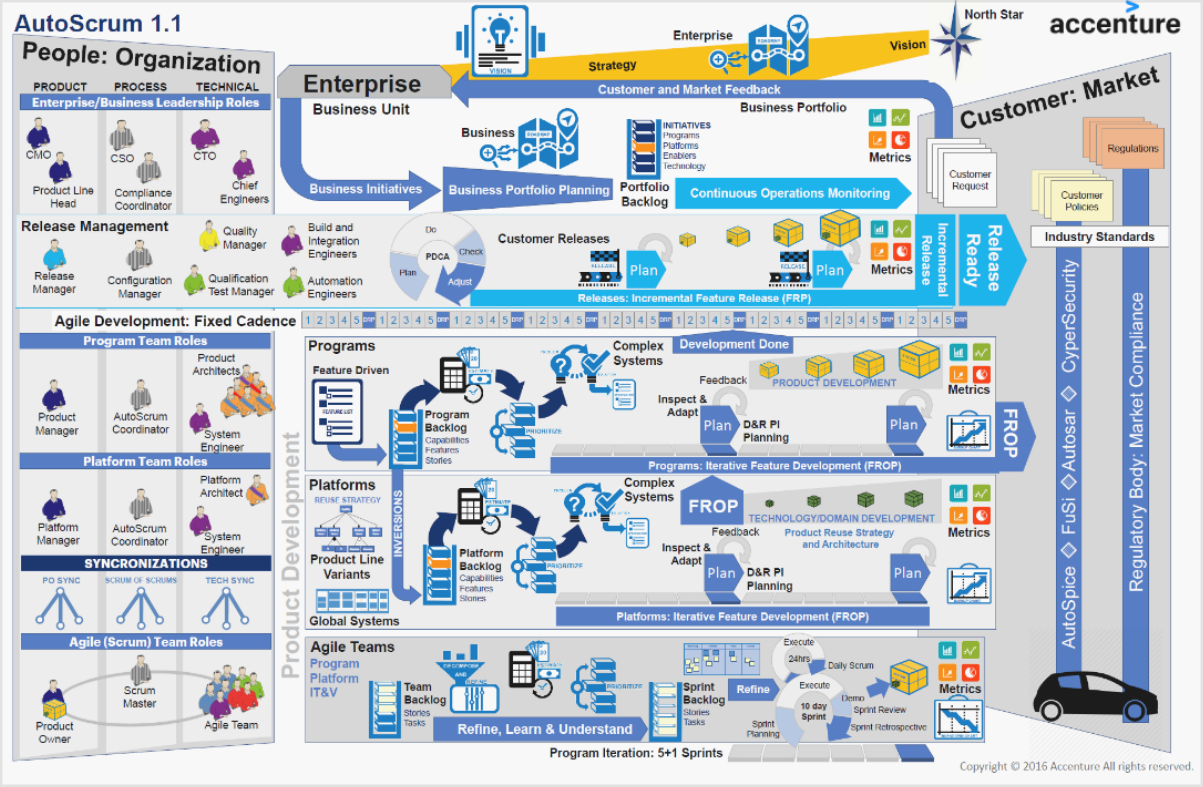
\includegraphics[width=\textwidth]{autoscrum.png}
  \caption{Excerpt from the presentation "AGILE TRANSFORMATION? FOR COMPLEX SYSTEMS? ...NO WAY!" by Brehm \cite{brehmAGILETRANSFORMATIONCOMPLEX2025} showing the Autoscrum framework.}
  \label{fig:autoscrum}
\end{figure}

\begin{figure}
  \centering
  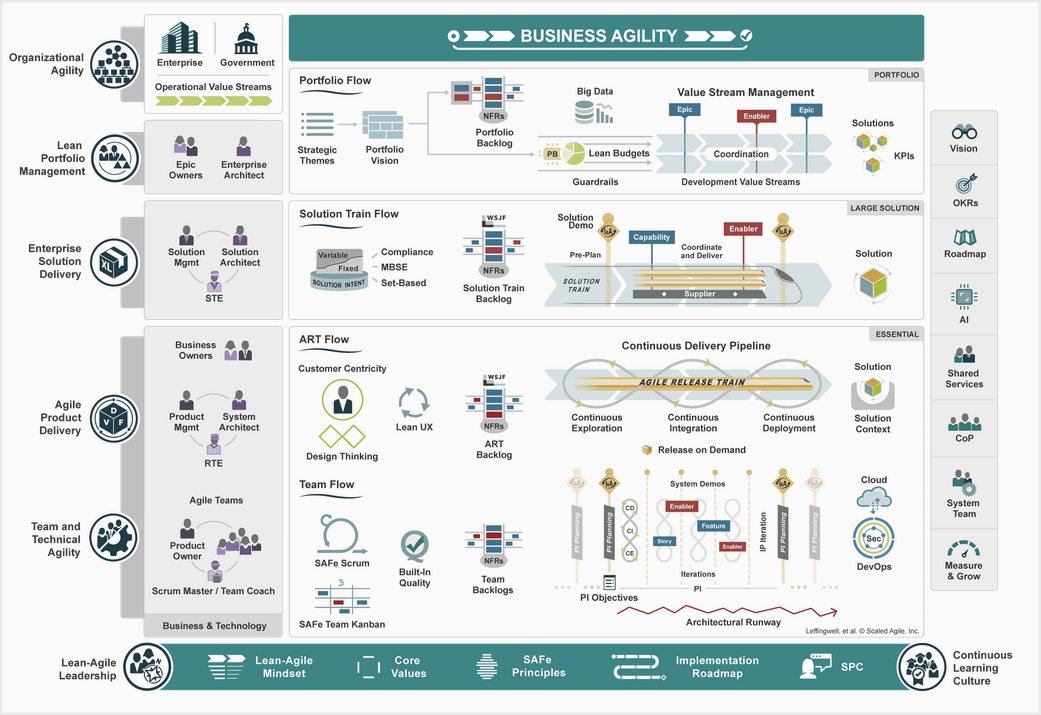
\includegraphics[width=\textwidth]{sAFE.png}
  \caption{The Scaled Agile Framework (SAFe) \cite{Framework}.}
  \label{fig:sAFE}
\end{figure}

\begin{figure}
  \centering
  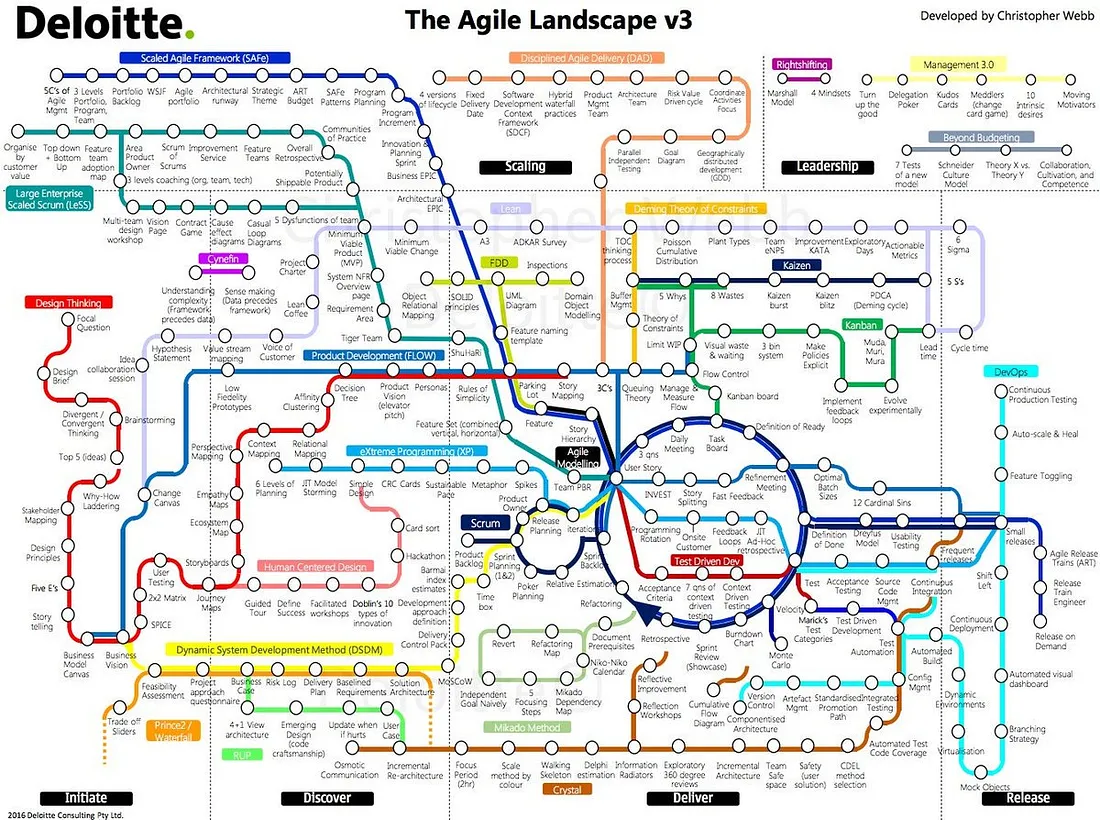
\includegraphics[width=\textwidth]{the_agile_landscape.png}
  \caption{The Agile Landscape v3 \cite{DeloitteAuditConsulting} showing the different frameworks and methods used for project management.}
  \label{fig:the_agile_landscape}
\end{figure}

\newpage

\subsection{Kanban}
\subsection{Waterfall}
\subsection{Extreme Programming}
\subsection{DevOps}

\section{NETCONF and YANG sensor management}

Hardware management is an essential part of administrating a larger network. Together with Lightside Instruments we have 
developed open source tools for YANG and NETCONF aimed at hardware sensor management.


\subsection{YANG Model}
The YANG model is a model used to describe the state and actions of a NETCONF device.
The Internet Engineering Task Force (IETF) has developed a set of standard YANG models for NETCONF devices.
For the purposes of this project we will not be using the standard YANG models,
but instead we will be using a custom YANG model developed by Lightside Instruments AS that only 
describes the state of thermometers. See \textit{Figure \ref{fig:yang}} for the YANG model.
\begin{figure}
  \begin{verbatim}
    module lsi-thermometers {
      yang-version 1.1;
      namespace "urn:lsi:params:xml:ns:yang:thermometers";
      prefix thermometers;

      organization  "Lightside Instruments AS";

      description
        "Thermometers monitoring module.";

      revision 2022-07-25 {
        description
          "Initial version.";
      }

      container thermometers {
        config false;
        list thermometer {
          key "name";
          leaf name {
            type string;
          }
          leaf value {
            description
              "Temperature in degrees Celsius multiplied by 100.";
            type int32 {
              range "-27315..max";
            }
          }
        }
      }
    }
  \end{verbatim}
  \caption{YANG model for thermometer management}
  \label{fig:yang}
\end{figure}

\newpage

\subsection{Node-RED}
Node-RED is a low code programming tool for event driven applications.
It makes it possible to create arbitrary flows that function as a compatibility layer
between different systems and protocols. The low code nature of Node-RED makes arbitrary system
integration accessible even for the lay person.

\subsubsection{Red-Netconf}
Red-Netconf \cite{LightsideinstrumentsRednetconf} is a Node-RED plugin that implements the following two 
nodes:
\begin{itemize}
  \item \textbf{Netconf Session}: This node is used to create a NETCONF session with a NETCONF device.
  \item \textbf{Netconf Yangcli}: This node is used to send NETCONF commands to a NETCONF device using yangcli commands.
\end{itemize}
Using these two nodes we are able to create Node-RED flows that can manage NETCONF devices.

\subsubsubsection{Temperature alert}
As an example of how the Red-Netconf nodes can be used we created
a Node-RED reference flow that collects data from a thermometer and switches on an LED
when the temperature is above 25 degrees Celsius, this can be seen in \textit{Figure \ref{fig:red-netconf}}.

\newpage

\begin{figure}
  \centering
  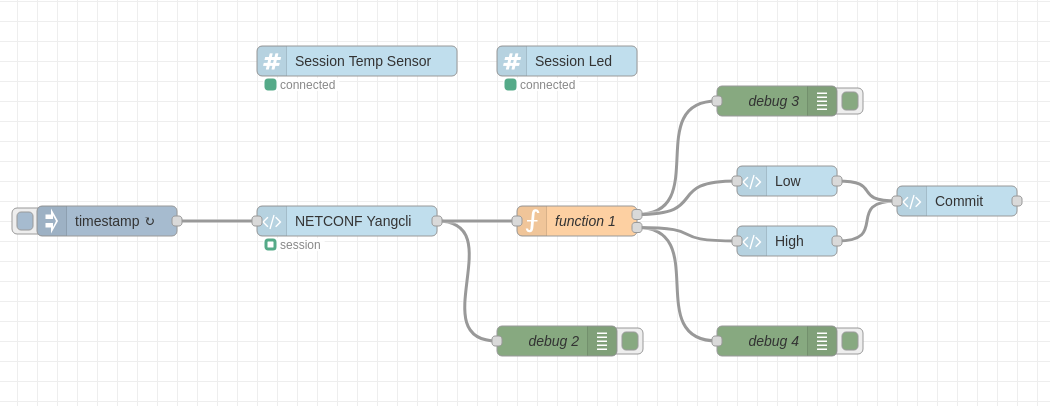
\includegraphics[width=\textwidth]{red-netconf.png}
  \caption{Node-RED flow using Red-Netconf nodes that monitors a temperature sensor and 
  switches on an LED when the temperature is above 25 degrees Celsius.}
  \label{fig:red-netconf}
\end{figure}


\subsubsection{Node-Yuma123}
Node-Yuma123 \cite{Nodeyuma1232025} is a NodeJS package that implements a set of Yuma123 bindings.


\subsubsubsection{easyNetconf}

\subsection{Grafana}

\section{NETCONF Security}

\pagebreak
\addcontentsline{toc}{section}{References}
\printbibliography
\license
\end{document}
